\setchapterabstract{本章阐明Why this course exists,回顾从 Pre-neural 到大型 Foundation Models 的 industrialization 演进;总结可迁移至 frontier models 的三大核心要素:mechanics、mindset、intuition;并对比 Character、Byte、Word 与 BPE 四种tokenizer方法。}

\vspace{-10cm}
\chapter{Overview and Tokenization}

\vspace{-2cm}

%%%%%%INSERT TOC BELOW 1ST SECTION%%%%%%%%%%%%

{\chaptoc\noindent\begin{minipage}[inner sep=0,outer sep=0]{0.9\linewidth}\section{Why this course exists}\end{minipage}}
\\
Problem: researchers are becoming {\color{tred}\textbf{disconnected}} from the underlying technology.

8 years ago, researchers would implement and train their own models.

6 years ago, researchers would download a model (e.g., BERT) and fine-tune it.

Today, researchers just prompt a {\color{tred}\textbf{proprietary}} model (e.g., GPT-4/Claude/Gemini).\\

Moving up levels of abstractions boosts productivity, but
\begin{itemize}
    \item These abstractions are \textbf{leaky} (in contrast to programming languages or operating systems).
    \item There is still fundamental research to be done that require \textbf{tearing up the stack}.
\end{itemize}


\Remark{Full understanding of this technology is necessary for fundamental research.
}

\subsection{The industrialization of language models
}
% 图 1:OPT FLOPs 构成
\MarginImageWithNote
  {figs/lec1/lec1.01.png}
  {\captionof{figure}{fraction of FLOPs spent in attention versus MLP changes with scale.}}
  {%
    随着模型从 760M 增至 175B,单次更新的总 FLOPs 从 $4.3\times10^{15}$ 增至 $2.4\times10^{18}$。其中 FFN 部分占比由 44\% 上升到 80\%,而MHA则从约 50\% 下降到约 20\%,Logits 层开销可忽略。%
  }

% 图 2:能力突现
\MarginImageWithNote
  {figs/lec1/lec1.02.png}
  {\captionof{figure}{Emergent Abilities of Large Language Models}}
  {%
    在约 $10^{23}\sim10^{24}$ FLOPs 的规模阈值后,模型多项任务的表现会突然从随机水平跃升,体现了大模型的“质变”能力。%
  }

Frontier models are out of reach for us. But building small language models (<1B parameters in this class) might not be representative of large language models.

\Example{More is different}{
  \vspace{-0.7cm}
  \begin{enumerate}
    \item 
    Example 1: fraction of FLOPs spent in attention versus MLP changes with scale.
    \item 
    Example 2: emergence of behavior with scale.
  \end{enumerate}
}


\Definition{FLOPs vs FLOPS\label{def:FLOPs-FLOPS}
}
{FLOPs: Floating Point Operations; \\
FLOPS: Floating Point Operations per Second}

FLOPs: Floating Point Operations
\begin{itemize}
    \item 浮点运算次数,用来衡量模型计算的复杂度
    \item 更准确地说,它是指模型在进行一次前向传播过程中所需要的浮点运算总数,例如加法、减法、乘法、除法等。
    \item FLOPs 是一个模型本身的属性,与硬件无关,可以用来比较不同模型之间的计算量大小。 FLOPs 越小,通常意味着模型越轻量,计算速度越快,对资源的需求也越低。
\end{itemize}

FLOPS: Floating Point Operations per Second
\begin{itemize}
    \item 指的是每秒浮点运算次数,是衡量计算机或处理器浮点运算速度的指标。
    \item 它表示了硬件的计算能力,例如GPU 的算力,可以理解为硬件每秒能进行多少次浮点运算。FLOPS 越大,通常意味着硬件的计算速度越快,能够更快地完成模型的计算任务。
    \item 例如,一个高性能GPU 可能具有几TFLOPS (Tera FLOPS) 的算力,表示每秒可以进行几万亿次的浮点运算。
\end{itemize}

\subsection{What can we learn in this class that transfers to frontier models?
}
There are three types of knowledge:
    
\begin{itemize}
    \item Mechanics: how things work (what a Transformer is, how model parallelism leverages GPUs)
    \item Mindset: squeezing the most out of the hardware, taking scale seriously (scaling laws)
    \item Intuitions: which data and modeling decisions yield good accuracy
\end{itemize}

\Remark{Wrong interpretation: scale is all that matters, algorithms don't matter. \\ Right interpretation: \textbf{algorithms that scale is what matters.}}

\vspace{-0.5\baselineskip}  % 负值越大距离越小
\[
  \text{\textbf{accuracy}} = \text{\textbf{efficiency}} \times \text{\textbf{resources}}
\]

\Example{Efficiency is way more important at larger scale
}{\href{https://arxiv.org/abs/2005.04305}{Measuring the Algorithmic Efficiency of Neural Networks} showed 44x algorithmic efficiency on ImageNet between 2012 and 2019}


\clearpage

{\chaptoc\noindent\begin{minipage}[inner sep=0,outer sep=0]{0.9\linewidth}\section{Current Landscape}\end{minipage}}

\subsection*{Pre-neural (before 2010s)}
\begin{itemize}[leftmargin=*]
  \item Language model to measure the entropy of English (\href{https://en.wikipedia.org/wiki/Prediction_and_entropy_of_printed_English}{Shannon 1950})
  \item Lots of work on n-gram language models (for MT, speech recognition) (\href{https://www.aclweb.org/anthology/P07-2045/}{Brants et al. 2007})
\end{itemize}

\subsection*{Neural ingredients (2010s)}
\begin{itemize}[leftmargin=*]
  \item First neural language model (\href{https://www.jmlr.org/papers/volume3/bengio03a/bengio03a.pdf}{Bengio et al. 2003})
  \item Sequence-to-sequence modeling (for MT) (\href{https://papers.nips.cc/paper/5346-sequence-to-sequence-learning-with-neural-networks}{Sutskever et al. 2014})
  \item Adam optimizer (\href{https://arxiv.org/abs/1412.6980}{Kingma \& Ba 2014})
  \item Attention mechanism (for MT) (\href{https://arxiv.org/abs/1409.0473}{Bahdanau et al. 2014})
  \item Transformer architecture (for MT) (\href{https://arxiv.org/abs/1706.03762}{Vaswani et al. 2017})
  \item Mixture of experts (\href{https://arxiv.org/abs/1701.06538}{Shazeer et al. 2017})
  \item Model parallelism (\href{https://arxiv.org/abs/1811.06965}{Huang et al. 2018}, \href{https://arxiv.org/abs/1909.08053}{Rajbhandari et al. 2019}, \href{https://arxiv.org/abs/1909.08053}{Shoeybi et al. 2019})
\end{itemize}

\subsection*{Early foundation models (late 2010s)}
\begin{itemize}[leftmargin=*]
  \item ELMo: pretraining with LSTMs, fine-tuning helps tasks (\href{https://arxiv.org/abs/1802.05365}{Peters et al. 2018})
  \item BERT: pretraining with Transformer, fine-tuning helps tasks (\href{https://arxiv.org/abs/1810.04805}{Devlin et al. 2018})
  \item Google's T5 (11B): cast everything as text-to-text (\href{https://arxiv.org/abs/1910.10683}{Raffel et al. 2019})
\end{itemize}

\subsection*{Embracing scaling, more closed}
\begin{itemize}[leftmargin=*]
  \item OpenAI's GPT-2 (1.5B): fluent text, first signs of zero-shot, staged release (\href{https://cdn.openai.com/better-language-models/language_models_are_unsupervised_multitask_learners.pdf}{Radford et al. 2019})
  \item Scaling laws: provide hope/predictability for scaling (\href{https://arxiv.org/abs/2001.08361}{Kaplan et al. 2020})
  \item OpenAI's GPT-3 (175B): in-context learning, closed (\href{https://arxiv.org/abs/2005.14165}{Brown et al. 2020})
  \item Google's PaLM (540B): massive scale, undertrained (\href{https://arxiv.org/abs/2204.02311}{Chowdhery et al. 2022})
  \item DeepMind's Chinchilla (70B): compute-optimal scaling laws (\href{https://arxiv.org/abs/2203.15556}{Hoffmann et al. 2022})
\end{itemize}

\subsection*{Open models}
\begin{itemize}[leftmargin=*]
  \item EleutherAI's open datasets (The Pile) and models (GPT-J) (\href{https://arxiv.org/abs/2101.00027}{Gao et al. 2020}, \href{https://arxiv.org/abs/2104.08691}{Wang et al. 2021})
  \item Meta's OPT (175B): GPT-3 replication, hardware issues (\href{https://arxiv.org/abs/2205.01068}{Zhang et al. 2022})
  \item Hugging Face/BigScience's BLOOM: focused on data sourcing (\href{https://arxiv.org/abs/2211.05100}{Workshop et al. 2022})
  \item Meta's Llama models (\href{https://arxiv.org/abs/2302.03781}{Touvron et al. 2023}, \href{https://arxiv.org/abs/2305.00000}{Touvron et al. 2023b}, \href{https://arxiv.org/abs/2403.00000}{Grattafiori et al. 2024})
  \item Alibaba's Qwen models (\href{https://arxiv.org/abs/2401.00000}{Qwen et al. 2024})
  \item DeepSeek's models (\href{https://example.com/deepseek-2024a}{DeepSeek-AI 2024a}, \href{https://example.com/deepseek-2024b}{DeepSeek-AI 2024b}, \href{https://example.com/deepseek-2024c}{DeepSeek-AI 2024c})
  \item AI2's OLMo 2 (\href{https://example.com/olmo2-2024}{Groeneveld et al. 2024}, \href{https://example.com/olmo2b-2024}{OLMo 2024})
\end{itemize}

\subsection*{Levels of openness}
\begin{description}[leftmargin=*]
  \item[Closed models] (e.g., GPT-4o): API access only (\href{https://openai.com/product/gpt-4o}{OpenAI 2023})
  \item[Open-weight models] (e.g., DeepSeek): weights + architecture details, no data details (\href{https://example.com/deepseek-2024a}{DeepSeek-AI 2024a})
  \item[Open-source models] (e.g., OLMo): weights, data, paper details (\href{https://example.com/olmo2-2024}{Groeneveld et al. 2024})
\end{description}

\subsection*{Today's frontier models}
\begin{itemize}[leftmargin=*]
  \item OpenAI's o3: \url{https://openai.com/index/openai-o3-mini/}
  \item Anthropic's Claude Sonnet 3.7: \url{https://www.anthropic.com/news/claude-3-7-sonnet}
  \item xAI's Grok 3: \url{https://x.ai/news/grok-3}
  \item Google's Gemini 2.5: \url{https://blog.google/technology/google-deepmind/gemini-model-thinking-updates-march-2025/}
  \item Meta's Llama 3.3: \url{https://ai.meta.com/blog/meta-llama-3/}
  \item DeepSeek's r1: \href{https://example.com/deepseek-2025}{DeepSeek-AI 2025}
  \item Alibaba's Qwen 2.5 Max: \url{https://qwenlm.github.io/blog/qwen2.5-max/}
  \item Tencent's Hunyuan-T1: \url{https://tencent.github.io/llm.hunyuan.T1/README_EN.html}
\end{itemize}

\clearpage
{\chaptoc\noindent\begin{minipage}[inner sep=0,outer sep=0]{0.9\linewidth}\section{Course Components}\end{minipage}}

\textbf{It's all about efficiency}

{\color{dblue} Resources: data + hardware (compute, memory, communication bandwidth)}

{\color{tred}How do you train the best model given a fixed set of resources?}
\subsection*{Design Decisions}

\begin{figure}[htbp]
  \centering
  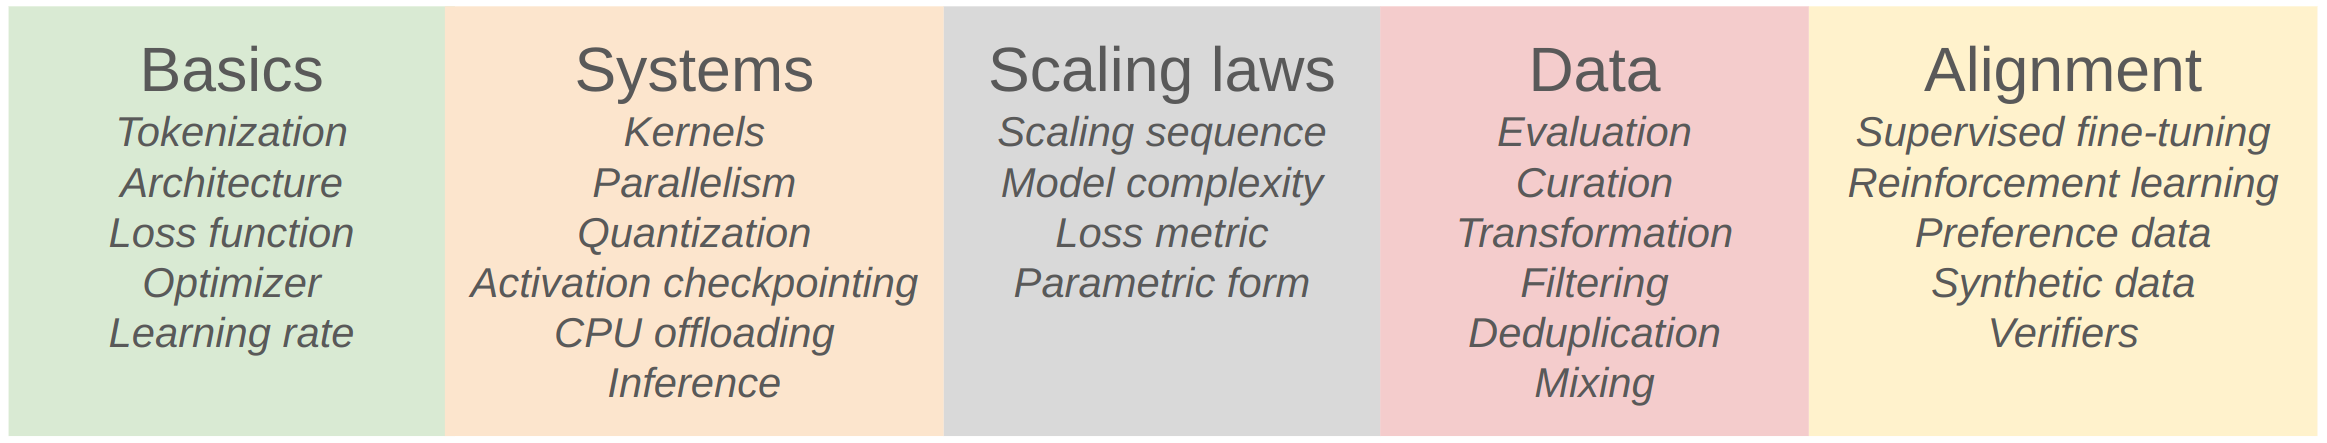
\includegraphics[width=1\linewidth]{figs/lec1/lec1.03.png}
  \caption{Design Decisions}
  \label{fig:design decisions}
\end{figure}


% 正文
\begin{itemize}[leftmargin=2cm]
  \item[Data processing]
  \begin{itemize}[leftmargin=0em,label={},noitemsep]
    \item 要点:丢弃“脏数据”或对任务无益的数据,避免浪费宝贵的计算资源去更新模型。
    \item 实践:在训练前做严格的数据清洗、筛选和质量评估,对噪声大样本打折扣或干脆丢弃。
  \end{itemize}

  \item[Tokenization]
  \begin{itemize}[leftmargin=0em,label={},noitemsep]
    \item 要点:虽然直接用原始字节(byte‐level)分词很优雅、简单,但会显著增加 token 数量,从而大幅提升计算量。
    \item 实践:通常改用 BPE、SentencePiece 等子词级方法,折衷“覆盖稀有词能力”与“token 数量”之间的算力开销。
  \end{itemize}

  \item[Model architecture]
  \begin{itemize}[leftmargin=0em,label={},noitemsep]
    \item 要点:为了减少内存和 FLOPs,许多网络结构和实现技巧应运而生。
    \item 实践:如 KV Cache 共享可在推理时节省重复计算,Sliding Window Attention 用局部窗口替代全局自注意力以降低复杂度。
  \end{itemize}

  \item[Training]
  \begin{itemize}[leftmargin=0em,label={},noitemsep]
    \item 要点:在超大规模数据和模型上,往往一轮(epoch)就够用了,因为数据量巨大,单轮已覆盖足够多样本。
    \item 实践:这样可以显著缩短训练时间,并提高算力利用效率。
  \end{itemize}

  \item[Scaling laws]
  \begin{itemize}[leftmargin=0em,label={},noitemsep]
    \item 要点:学习率、批大小等超参数在小模型上先调好,再“按比例”外推到大模型,可节省在巨型模型上反复调参的成本。
    \item 实践:先在上千万参数级别的模型上做超参网格搜索,再把最优设置直接拿去训练百亿参数级别的大模型。
  \end{itemize}

  \item[Alignment]
  \begin{itemize}[leftmargin=0em,label={},noitemsep]
    \item 要点:对齐(alignment)指将模型调教到用户期望的行为上。
    \item 影响:为更经济地满足对齐需求,通常先对小规模基础模型做微调,再逐步放大模型规模,而不在超大模型上从零开始对齐。
  \end{itemize}
\end{itemize}

\clearpage

\subsection{Basics}

\textbf{{\color{tred} Goal: get a basic version of the full pipeline working}}

\textbf{{\color{dblue} Components: tokenization, model architecture, training
}}
\subsubsection{Tokenization}
\MarginImageWithNote
  {figs/lec1/lec1.04.png}
  {\captionof{figure}{Tokenizer Example}}
  {Intuition: break up string into popular segments
  }
  
\Definition{Tokenization
}{Tokenizers convert between strings and sequences of integers (tokens)
}

\begin{itemize}[leftmargin=0em,label={},noitemsep]
  \item Byte-Pair Encoding (BPE) tokenizer: 
    \href{https://arxiv.org/abs/1508.07909}{Sennrich et al.\ 2015}
  \item Tokenizer-free approaches: 
    \href{https://arxiv.org/abs/2105.13626}{Xue et al.\ 2021}, 
    \href{https://arxiv.org/pdf/2305.07185.pdf}{Yu et al.\ 2023}, 
    \href{https://arxiv.org/abs/2412.09871}{Pagnoni et al.\ 2024}, 
    \href{https://arxiv.org/abs/2406.19223}{Deiseroth et al.\ 2024}
  \item Use bytes directly, promising, but have not yet been scaled up to the frontier.
\end{itemize}


\subsubsection{Architecture}
\MarginImageWithNote
  {figs/lec1/lec1.05.png}
  {\captionof{figure}{Transformer}}
  
Starting point: original Transformer \href{https://arxiv.org/pdf/1706.03762.pdf}{[Vaswani+ 2017]}

\vspace{1em}
\begin{itemize}[leftmargin=0em]
  \item Activation functions: ReLU, SwiGLU (\href{https://arxiv.org/pdf/2002.05202.pdf}{Shazeer 2020})
  \item Positional encodings: sinusoidal, RoPE (\href{https://arxiv.org/pdf/2104.09864.pdf}{Su et al.\ 2021})
  \item Normalization: LayerNorm, RMSNorm (\href{https://arxiv.org/pdf/1607.06450.pdf}{Ba et al.\ 2016}, \href{https://arxiv.org/abs/1910.07467}{Zhang et al.\ 2019})
  \item Placement of normalization: pre-norm versus post-norm (\href{https://arxiv.org/pdf/2002.04745.pdf}{Xiong et al.\ 2020})
  \item MLP: dense, mixture of experts (\href{https://arxiv.org/pdf/1701.06538.pdf}{Shazeer et al.\ 2017})
  
  \item Attention: full, sliding window, linear (\href{https://arxiv.org/pdf/2310.06825.pdf}{Jiang et al.\ 2023}, \href{https://arxiv.org/abs/2006.16236}{Katharopoulos et al.\ 2020})
  \item Lower-dimensional attention: group-query attention (GQA), multi-head latent attention (MLA) (\href{https://arxiv.org/pdf/2305.13245.pdf}{Ainslie et al.\ 2023}, \href{https://arxiv.org/abs/2405.04434}{DeepSeek-AI et al.\ 2024})
  \item State-space models: Hyena (\href{https://arxiv.org/abs/2302.10866}{Poli et al.\ 2023})
\end{itemize}

\subsubsection{Training}

\begin{itemize}[leftmargin=0em,label=\textbullet]
\item Optimizer (e.g., AdamW, Muon, SOAP):
\href{https://arxiv.org/abs/1412.6980}{Kingma et al.\ 2014},
\href{https://arxiv.org/abs/1711.05101}{Loshchilov et al.\ 2017},
\href{https://kellerjordan.github.io/posts/muon/}{Keller 2024},
\href{https://arxiv.org/abs/2409.11321}{Vyas et al.\ 2024}
\item Learning rate schedule (e.g., cosine, WSD):
\href{https://arxiv.org/pdf/1608.03983.pdf}{Loshchilov et al.\ 2016},
\href{https://arxiv.org/pdf/2404.06395}{Hu et al.\ 2024}
\item Batch size (e.g., critical batch size):
\href{https://arxiv.org/pdf/1812.06162.pdf}{McCandlish et al.\ 2018}
\item Regularization (e.g., dropout, weight decay)
\item Hyperparameters (number of heads, hidden dimension): grid search
\end{itemize}

\clearpage 
\subsection{Systems}

\textbf{{\color{tred} Goal: squeeze the most out of the hardware}}

\textbf{{\color{dblue} Components: kernels, parallelism, inference
}}
\subsubsection{Kernels}

\MarginImageWithNote
  {figs/lec1/lec1.06.png}
  {\captionof{figure}{GPU Kernels}}
  {SM: Streaming Multiprocessor -- 并行运算核心\\ 一个 SM 内含数十到上百个 CUDA 核心(CUDA Cores),它们同时执行浮点或整数运算。}
  
\begin{figure}[ht]
  \centering
  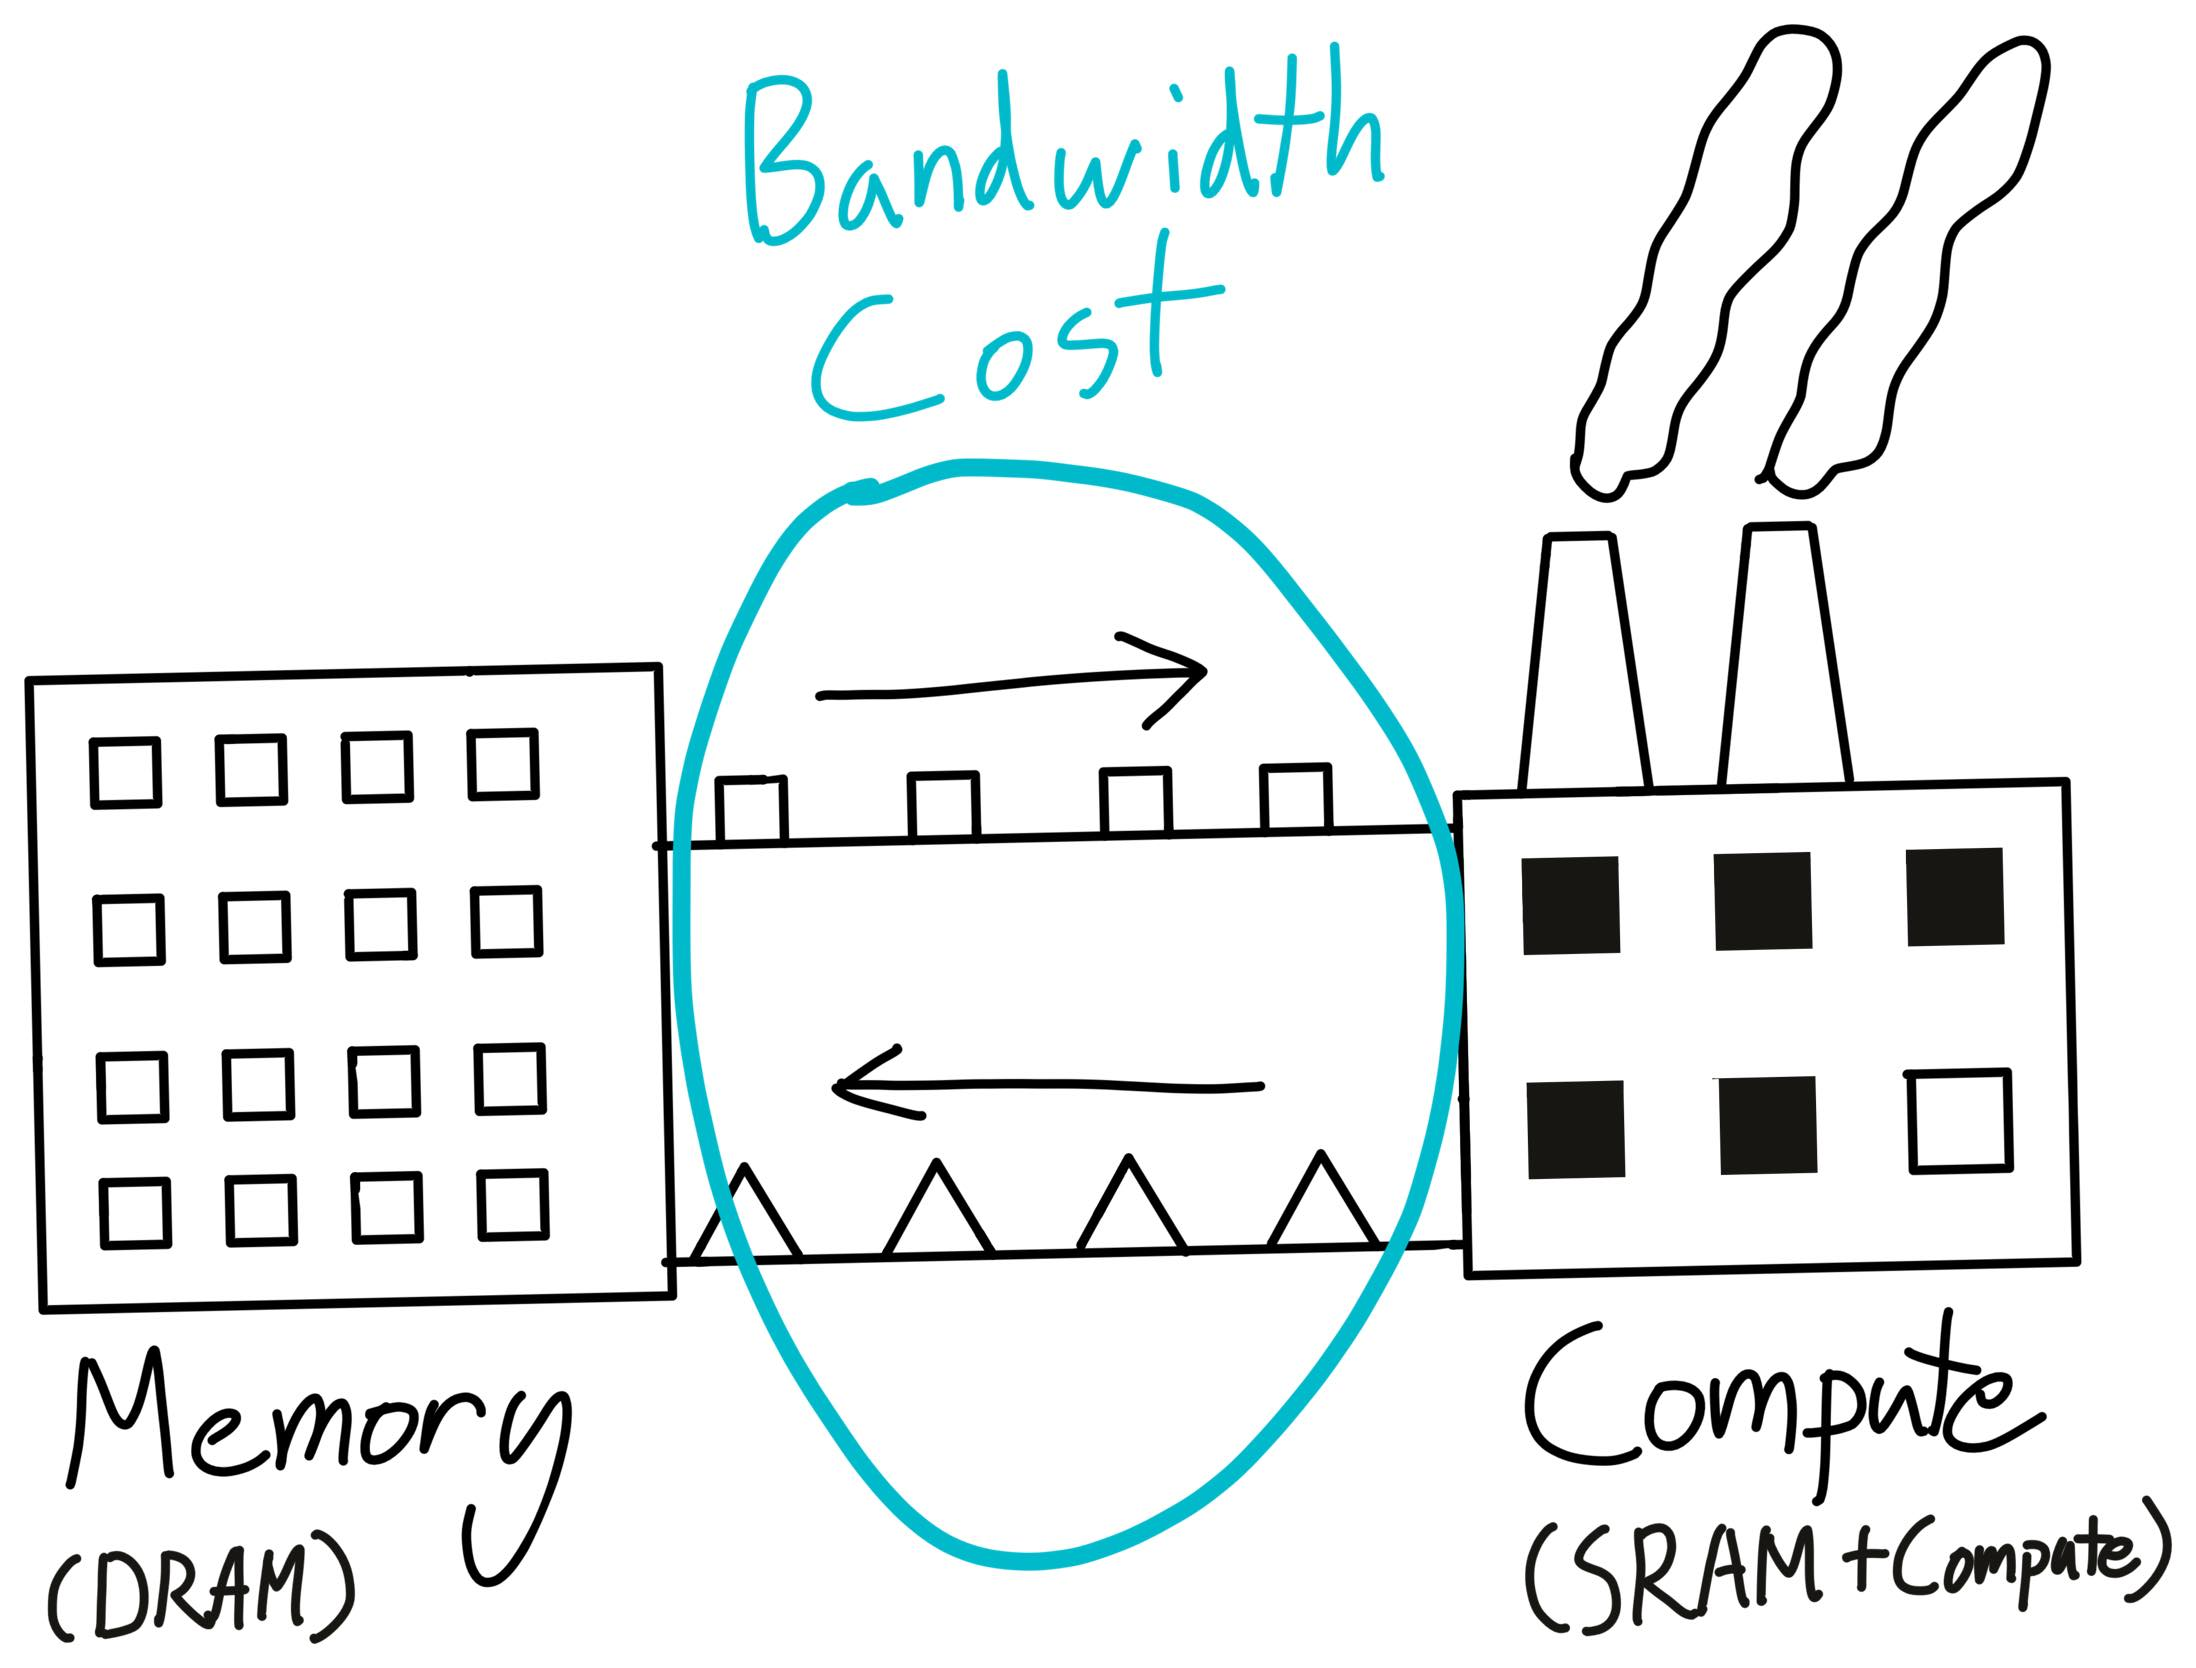
\includegraphics[width=0.8\textwidth]{figs/lec1/lec1.07.png}
  \caption{Memory 与 Compute之间的数据传输带宽开销示意}
  \label{fig:bandwidth-cost}
\end{figure}

Analogy: warehouse : DRAM :: factory : SRAM

\begin{itemize}[leftmargin=*]
  \item DRAM(动态随机存取存储器)
    \begin{itemize}[leftmargin=1.5em,noitemsep]
      \item 特点:高密度、成本低,但访问延迟较高且功耗受刷新影响。
      \item 用途:作为系统主存,用于存放大规模数据。
    \end{itemize}

  \item SRAM(静态随机存取存储器)
    \begin{itemize}[leftmargin=1.5em,noitemsep]
      \item 特点:访问速度极快(几纳秒)、带宽高,但密度低、成本和静态功耗都较高。
      \item 用途:作为 CPU/GPU 的一级/二级缓存与寄存器文件,提供高速数据访问。
    \end{itemize}

  \item 带宽开销(Bandwidth Cost)
    \begin{itemize}[leftmargin=1.5em,noitemsep]
      \item 定义:单位时间内从 DRAM 到 Compute 或反向传输数据所能达到的最大量,以及对应的能量消耗。
      \item 影响:DRAM 带宽一般在几十到数百 GB/s,而 SRAM 缓存内部带宽可达 TB/s 级别。带宽越大、延迟越低,能更好地支撑高并行度计算;但高带宽存储往往成本和功耗也更高。
      \item 优化策略:数据重用、批量传输(coalescing)、压缩/量化,以及层次化缓存设计,都是为降低带宽开销、提升整体吞吐而常用的手段。
    \end{itemize}
\end{itemize}

\Remark{Trick: organize computation to maximize utilization of GPUs by minimizing data movement}

Write kernels in CUDA/\textbf{Triton}/CUTLASS/ThunderKittens


\subsubsection{Parallelism}
{\color{tred}Data movement between GPUs is even slower, but same \textbf{'minimize data movement' principle holds}.}

\begin{itemize}[leftmargin=*]
  \item Use collective operations (e.g., gather, reduce, all-reduce)
    \begin{itemize}[leftmargin=0em, noitemsep]
      \item \textbf{gather}:将各 GPU 的局部结果聚合到一个设备上,适用于收集梯度或特定张量。
      \item \textbf{reduce}:在所有设备上对张量执行聚合(如求和、最大值),并将结果保存在一个设备。
      \item \textbf{all-reduce}:在所有设备上对张量聚合,且将聚合结果广播给每个设备,常用来同步梯度。
    \end{itemize}

  \item Shard (parameters, activations, gradients, optimizer states) across GPUs
    \begin{itemize}[leftmargin=0em, noitemsep]
      \item 参数分片:将模型参数切分到不同 GPU,减少单卡显存压力。
      \item 激活值分片:训练时将中间激活存储分配到多卡,缓解显存占用高峰。
      \item 梯度分片:反向传播时只聚合本卡分片梯度,减少通信量。
      \item 优化器状态分片:将动量、二阶矩等优化器状态分散存储,节省缓存空间。
    \end{itemize}

  \item How to split computation: \{data, tensor, pipeline, sequence\} parallelism
    \begin{itemize}[leftmargin=0em, noitemsep]
      \item 数据并行(Data parallelism):每卡保留完整模型,输入数据分批到各卡并行计算,梯度通过 all-reduce 同步。
      \item 张量并行(Tensor parallelism):将单层中大矩阵乘法拆分到多卡(按行/列切分),并行执行。
      \item 流水线并行(Pipeline parallelism):将模型按层切分成多个阶段,不同 GPU 串行执行各自阶段,并以微批实现并发。
      \item 序列并行(Sequence parallelism):对长序列输入按段切分,在各卡并行处理不同序列片段,适用于超长上下文场景。
    \end{itemize}
\end{itemize}

    
\subsubsection{Inference}

\textbf{{\color{tred}Goal: generate tokens given a prompt (needed to actually use models!)}}

Inference is also needed for reinforcement learning, test-time compute, evaluation

Globally, inference compute (every use) exceeds training compute (one-time cost)

\hl{Two phases: prefill and decode}\\

\MarginImageWithNote
  {figs/lec1/lec1.08.png}
  {\captionof{figure}{Inference}}
  
\vspace{1em}

\begin{itemize}
    \item Prefill (similar to training): tokens are given, can process all at once (compute-bound)
    \\
    Take the prompt, and can run it through the model and get some activation.
    \item Decode: need to generate one token at a time (memory-bound)\\
    Go autoregressively one by one and generate tokens.
\end{itemize}

\vspace{1em}

Methods to speed up decoding:
    \begin{enumerate}
        \item Use cheaper model (via model pruning, quantization, distillation)
        \item Speculative decoding: use a cheaper "draft" model to generate multiple tokens, then use the full model to score in parallel (exact decoding!)
        \item Systems optimizations: KV caching, batching
    \end{enumerate}

\subsection{Scaling Laws}
\textbf{{\color{tred} Goal: do experiments at small scale, predict hyperparameters/loss at large scale
}}

Question: given a FLOPs budget ($C$), use a bigger model ($N$) or train on more tokens ($D$)?

Compute-optimal scaling laws: $D = 20 N$ (e.g., 1.4B parameter model should be trained on 28B tokens)

\begin{figure}[ht]
  \centering
  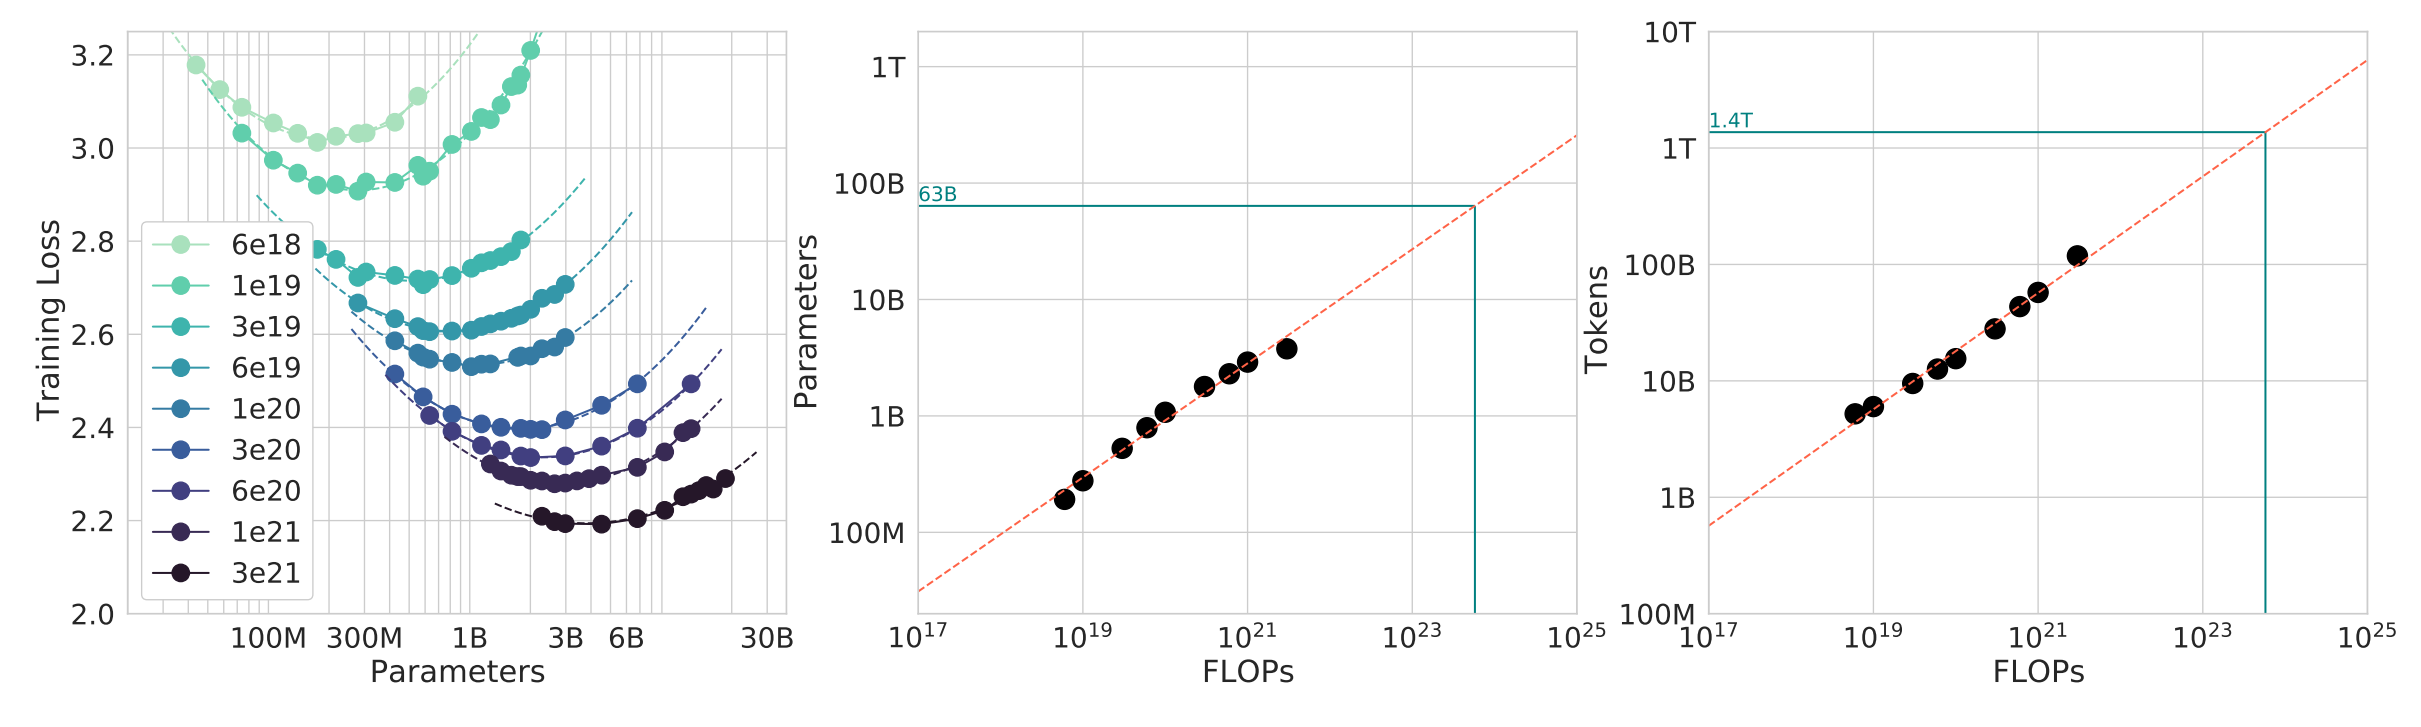
\includegraphics[width=0.8\textwidth]{figs/lec1/lec1.09.png}
  \caption{Scaling Laws}
  \label{fig:scaling laws}
\end{figure}


\subsection{Data}

Question: What capabilities do we want the model to have?

Multilingual? Code? Math?
\begin{figure}[ht]
  \centering
  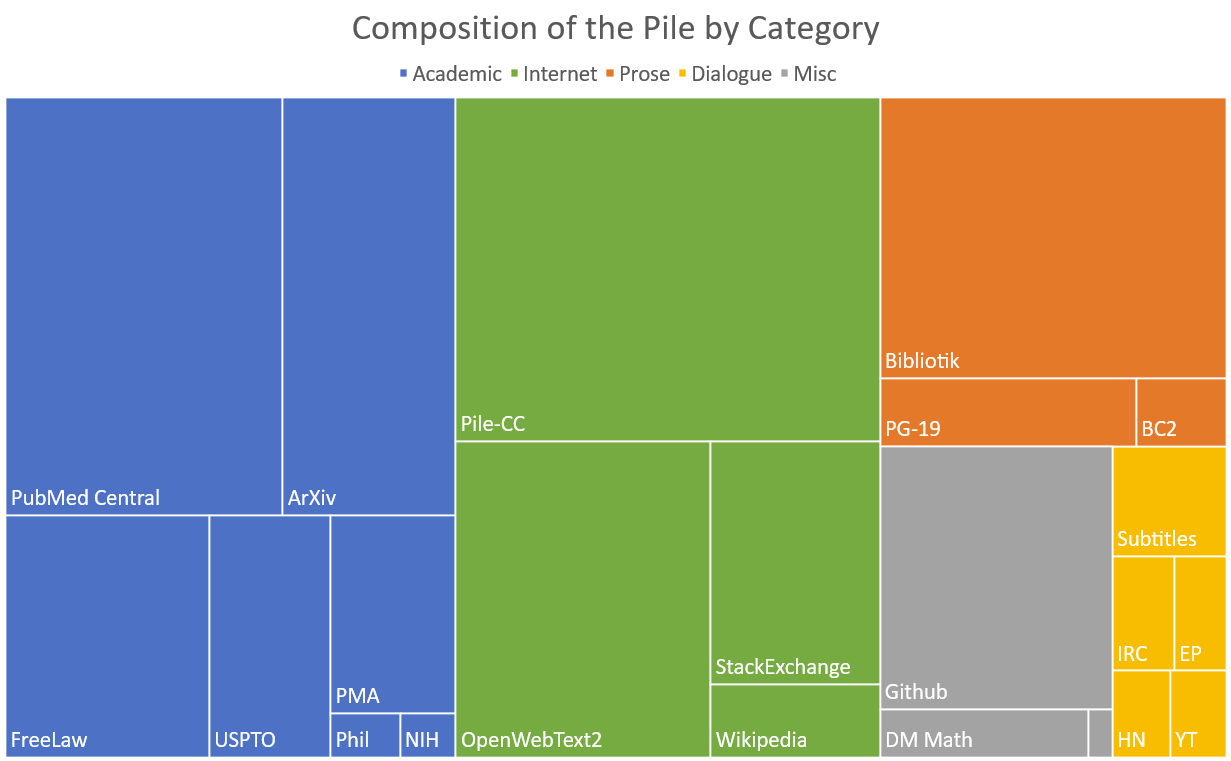
\includegraphics[width=0.8\textwidth]{figs/lec1/lec1.11.png}
  \caption{Composition of Data}
  \label{fig:data}
\end{figure}

\vspace{-3em}

\subsubsection{Evaluation}
\begin{itemize}[leftmargin=*]
  \item Perplexity: 教科书式的语言模型评价指标,用于衡量模型对下一个 token 的预测能力,值越低越好。
  \item Standardized testing: 使用 MMLU、HellaSwag、GSM8K 等测试集评估模型的知识掌握、常识推理与数学能力。
  \item Instruction following: 通过 AlpacaEval、IFEval、WildBench 等基准测试模型对人类指令的响应与执行效果。
  \item Scaling test-time compute: 在推理阶段额外使用 chain-of-thought(链式思维提示)和模型集成等技术,以提高推理质量。
  \item LM-as-a-judge: 用另一个语言模型对生成结果进行质量评判,度量文本的连贯性与正确性。
  \item Full system: 评估包含检索增强生成(RAG)和智能 agent 的完整系统时,需要考虑端到端的交互与任务完成效果。
\end{itemize}

\subsubsection{Data curation}
\begin{itemize}[leftmargin=*]
  \item “数据不会从天而降”:需要主动设计爬虫和采集管道(如 \texttt{look\_at\_web\_data()})来获取原始数据。
  \item 来源:网页抓取内容、图书、arXiv 论文、GitHub 代码等多种渠道。
  \item 法律合规:可依据 “公平使用” 原则(Henderson et al.\ 2023)训练,或与数据拥有者签订许可(如 Google 与 Reddit 的数据授权)。
  \item 格式多样:HTML、PDF、目录结构等都需要统一转换成可处理的文本格式。
\end{itemize}

  
\subsubsection{Data processing}
\begin{itemize}[leftmargin=*]
  \item Transformation: 将 HTML/PDF 转为纯文本,同时保留核心内容和必要的结构信息,必要时进行重写和清洗。
  \item Filtering: 使用分类器筛除低质量或有害内容,确保训练数据的可靠性与安全性。
  \item Deduplication: 利用 Bloom Filter、MinHash 等算法去重,既节省计算资源,又避免模型过度记忆重复样本。
\end{itemize}

对于真实的网页数据,通常是乱文,需要做很多处理。\href{例子}{https://stanford-cs336.github.io/spring2025-lectures/var/sample-documents.txt}

\subsection{Alignment}
So far, a base model is raw potential, very good at completing the next token. \textbf{Alignment makes the model actually useful.}    

{\color{tred}
Goals of alignment:
\textbf{Get the language model to follow instructions
Tune the style (format, length, tone, etc.)
Incorporate safety (e.g., refusals to answer harmful questions)}
}

Two phases:
    \begin{enumerate}
        \item supervised finetuning
        \item learning from feedback
    \end{enumerate}

\MarginImageWithNote
  {figs/lec1/lec1.12.png}
  {\captionof{figure}{SFT Code 示意}}
  {包含预设好的回答}

\paragraph{Supervised Fine-Tuning (SFT)}
\begin{itemize}[leftmargin=*]
  \item Instruction data: (prompt, response) pairs 
  \item Data often involves human annotation.
  \item Intuition: base model already has the skills, just need few examples to surface them (\href{https://arxiv.org/abs/2311.07911}{Zhou et al.\ 2023})
  \item Supervised learning: fine-tune model to maximize \(p(\text{response}\mid\text{prompt})\). 这里的response是用户已经提供作为微调的。
\end{itemize}

\clearpage
\paragraph{Learning from Feedback}
\MarginImageWithNote
  {figs/lec1/lec1.13.png}
  {\captionof{figure}{Learn from feedback示意 }}
  {系统返回两个回答,由用户选择}

\begin{itemize}[leftmargin=*]
  \item Preference data:
    \begin{itemize}[leftmargin=1em,label={},noitemsep]
      \item Data: generate multiple responses using model (e.g., [A, B]) to a given prompt.
      \item User provides preferences (e.g., A < B or A > B).
    \end{itemize}

  \item Verifiers:
    \begin{itemize}[leftmargin=1em,label={},noitemsep]
      \item Formal verifiers (e.g., for code, math).
      \item Learned verifiers: train against an LM-as-a-judge.
    \end{itemize}

  \item Algorithms:
    \begin{itemize}[leftmargin=1em,label={},noitemsep]
      \item Proximal Policy Optimization (PPO) (\href{https://arxiv.org/abs/1707.06347}{Schulman et al.\ 2017} , \href{https://arxiv.org/abs/2203.02155}{Ouyang et al.\ 2022} 
      \item Direct Preference Optimization (DPO) (\href{https://arxiv.org/abs/2305.18290}{Rafailov et al.\ 2023}) 
      \item Group Relative Preference Optimization (GRPO) (\href{https://arxiv.org/abs/2402.03300}{Shao et al.\ 2024}) 
    \end{itemize}
\end{itemize}
\clearpage

\phantomsection 
\hypertarget{lec1:tokenization}{}
{\chaptoc\noindent\begin{minipage}[inner sep=0,outer sep=0]{0.9\linewidth}\section{Tokenization}\end{minipage}}

\subsection{Intro}
Raw text is generally represented as \textbf{Unicode} strings.

A language model places a probability distribution over sequences of tokens (usually represented by integer indices).
    
So we need a procedure that {\color{tred}\textbf{encodes} strings into tokens.}

We also need a procedure that {\color{tred}\textbf{decodes} tokens back into strings.}

A  Tokenizer is a class that implements the encode and decode methods.

The vocabulary size is number of possible tokens (integers).

\subsection{Observations}

\begin{figure}[ht]
  \centering
  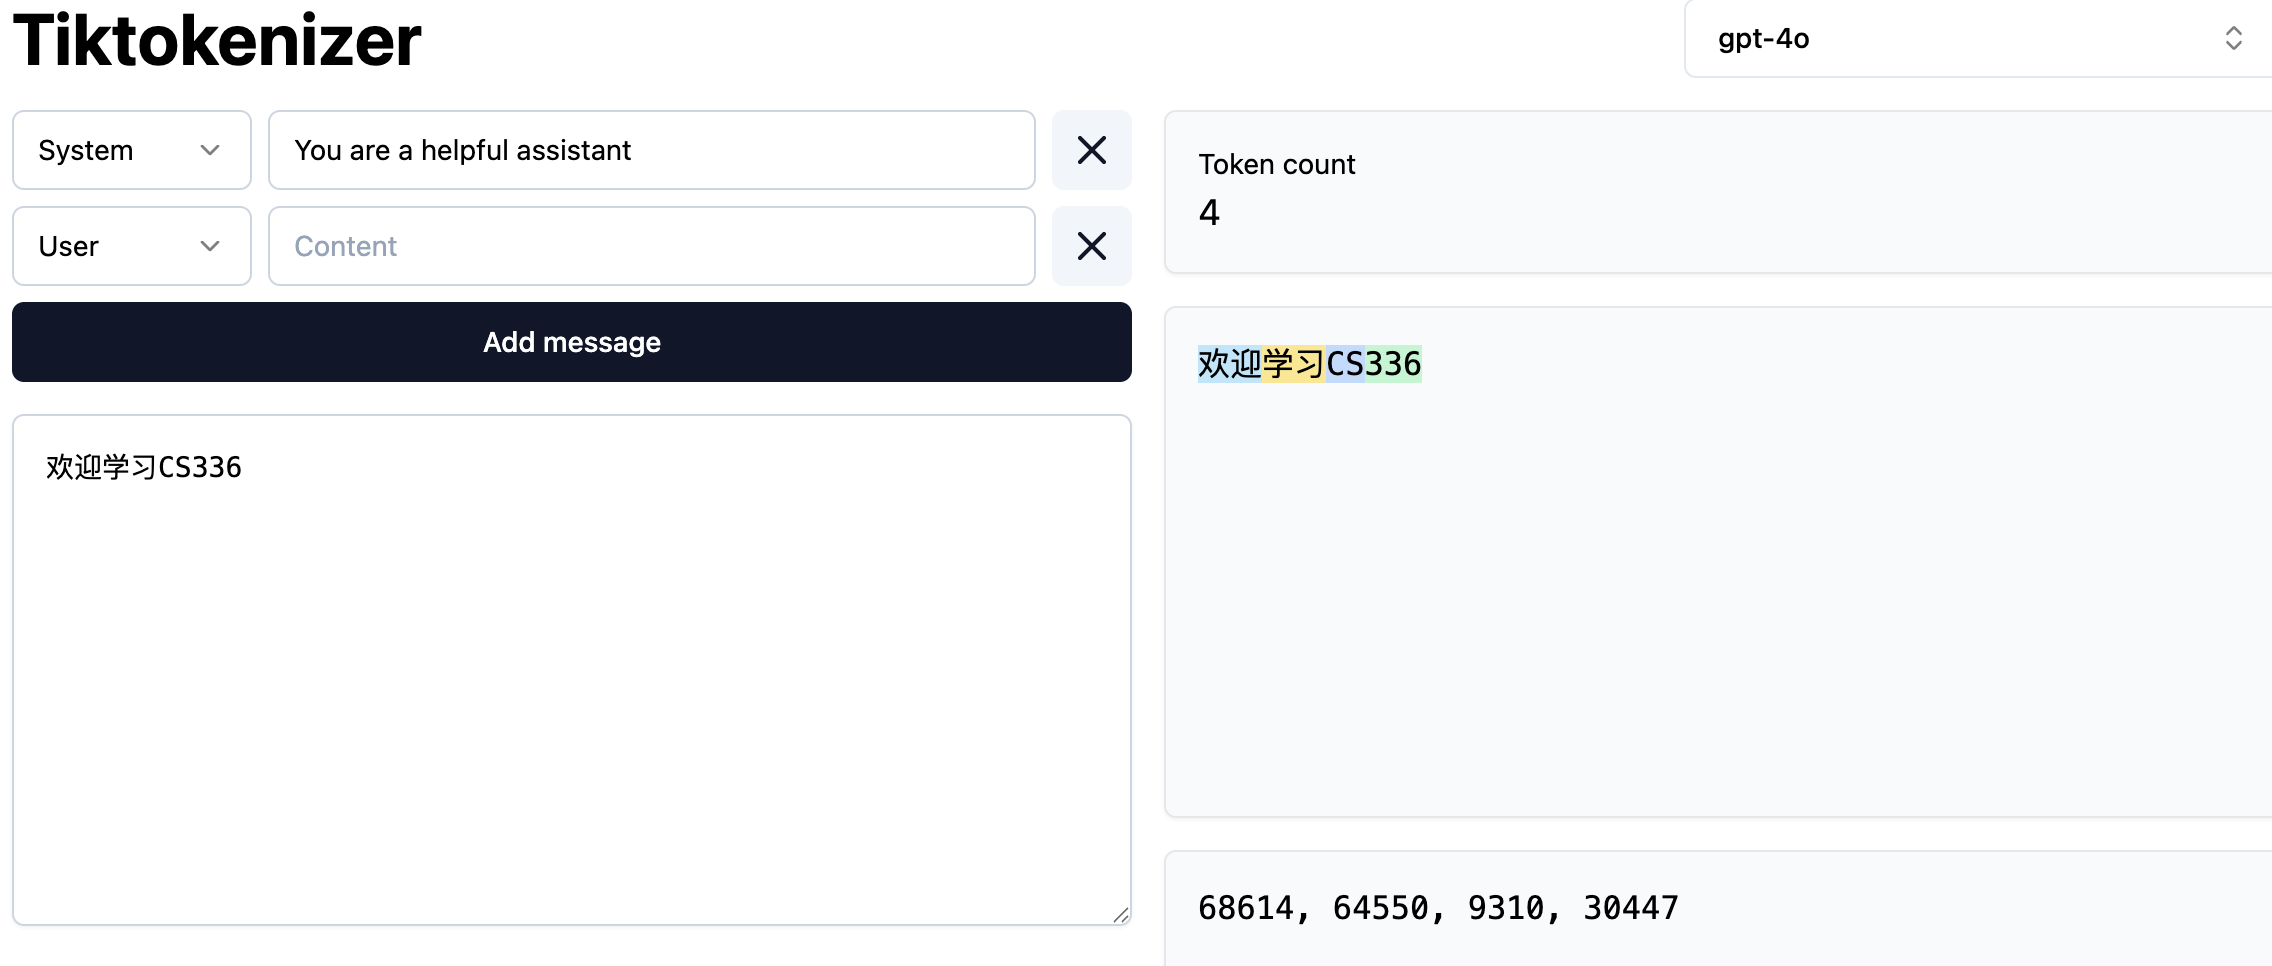
\includegraphics[width=0.8\textwidth]{figs/lec1/lec1.14.png}
  \caption{Tokenization}
  \label{fig:Tokenize}
\end{figure}

\MarginImageWithNote
  {figs/lec1/lec1.15.png}
  {\captionof{figure}{GPT-2 Tokenizer}}
  


\begin{itemize}
    \item A word and its preceding space are part of the same token (e.g., " world").
    \item A word at the beginning and in the middle are represented differently (e.g., "hello hello").
    \item Numbers are tokenized into every few digits.
\end{itemize}

\Definition{Compression Ratio}{
  \begin{itemize}[leftmargin=*]
    \item \(r = \displaystyle\frac{\text{num\_bytes}}{\text{num\_tokens}}
      = \frac{\lvert\texttt{bytes(string, 'utf-8')}\rvert}{\lvert\texttt{indices}\rvert}\)
    \item \(\text{num\_bytes} = \lvert\texttt{bytes(string, 'utf-8')}\rvert\),
      即字符串在 UTF-8 编码下的字节长度。
    \item \(\text{num\_tokens} = \lvert\texttt{indices}\rvert\),
      即分词后得到的 token 数量。
    \item 返回值 \(r\):表示每个 token 平均对应的字节数。
    \item 意义:
      \begin{itemize}[leftmargin=1em,noitemsep]
        \item 当 \(r\) 越大时,token 划分越“粗”,序列更短,每个 token 覆盖更多字节。
        \item 当 \(r\) 越小时,token 划分越“细”,序列更长,但表示更精细。
      \end{itemize}
  \end{itemize}
}

\subsection{Character Tokenizer}

\subsubsection*{Character-based Tokenization}

\MarginImageWithNote
  {figs/lec1/lec1.16.png}
  {\captionof{figure}{Character-based tokenization}}

A Unicode string is a sequence of Unicode characters.  

Each character can be converted to a code point (integer) via \texttt{ord}:
\begin{verbatim}
assert ord("a") == 97
\end{verbatim}
and converted back via \texttt{chr}:
\begin{verbatim}
assert chr(97) == "a"
\end{verbatim}


With Character-based tokenization, there are approximately 150{,}000 Unicode characters [Wikipedia], so the vocabulary size is
\[
  \text{vocab\_size} = \max(\text{indices}) + 1
\]
(This is a lower bound.)

\paragraph{Problems}
\begin{itemize}[leftmargin=*]
  \item Extremely large vocabulary (≈150K tokens).
  \item Many characters are very rare, leading to inefficient use of the token space.
\end{itemize}

\subsection{Byte Tokenizer}
\subsubsection*{Byte-level Tokenization}

\MarginImageWithNote
  {figs/lec1/lec1.17.png}
  {\captionof{figure}{Byte-based tokenization}}
  
Unicode strings can be represented as a sequence of bytes (integers 0–255). The most common encoding is UTF-8, where:

\begin{verbatim}
assert bytes("a", encoding="utf-8") == b"a"
\end{verbatim}

Now let's verify round-tripping with a byte tokenizer:

\begin{verbatim}
tokenizer = ByteTokenizer()
string    = "Hello! 你好!"
indices   = tokenizer.encode(string)
recon     = tokenizer.decode(indices)
assert string == recon
\end{verbatim}


\paragraph{Drawback}
\begin{itemize}[leftmargin=*]
  \item sequence length equals byte length, which is very long.
  \item Transformer context windows are limited and attention scales quadratically with length,  so this approach leads to prohibitive compute and memory costs.
\end{itemize}



\clearpage

\subsection{Word Tokenizer}

\MarginImageWithNote
  {figs/lec1/lec1.18.png}
  {\captionof{figure}{Word-based tokenization}}

  
Another approach (classic in NLP) is to split strings into words or subword-like segments:

To build a Tokenizer, map each segment to an integer ID via a lookup table.  

However, this method has drawbacks:

\paragraph{Drawback:}

\begin{itemize}[leftmargin=*]
  \item Vocabulary size grows with the number of distinct words—potentially very large (similar to Unicode code points). Vocabulary has a lot of tokens with minimal differences between them(e.g., apology, apologize, apologetic, apologist), which is resolved by {\color{dblue} \textbf{subword tokenization.}}
  \item Many words are rare, so the model sees them infrequently and learns little about them.
  \item There is no fixed vocabulary size.
\end{itemize}

\marginnote{ {\color{dblue} \textbf{Subword Tokenization}}: \\
This method contains full and partial words. \\
\textbf{Benefits:}\\
a.Vocabulary expressivity\\
b.Ability to represent new words by breaking down the new token into smaller characters which tend to be a part of the vocabulary.}


\noindent Vocabulary size:
\[
  \text{vocab\_size}
  = \text{number of distinct segments in the training data}
\]


\subsection{BPE Tokenizer}

Basic idea: train the tokenizer on \textbf{raw text} to automatically determine the vocabulary.

\Remark{Intuition: {\color{tred}common sequences} of characters are represented by a {\color{tred}single token}, {\color{dblue}rare sequences} are represented by {\color{dblue}many tokens}.}

The GPT-2 paper used word-based tokenization to break up the text into inital segments and run the original BPE algorithm on each segment.

\textbf{{\color{tred}Sketch: start with each byte as a token, and successively merge the most common pair of adjacent tokens.}}

\Remark{\color{tred}Recursively merges the most frequent pairs of consecutive bytes or characters in a corpus.}


\begin{algorithm}[htbp]
\caption{Byte $-$ Pair Encoding}\label{alg:bpe}
\KwIn{strings $C$, number of merges $k$}
\KwOut{vocabulary $V$}

$V \gets \{\text{all unique characters in }C\}$ \# initial set of tokens is characters\;

\For{$i\gets1$ \KwTo $k$}{
  $(t_L,t_R)\gets\arg\max_{(a,b)}\bigl|\{\,\text{adjacent }(a,b)\text{ in }C\}\bigr|$ \# most frequent pair\;
  $t_{\mathrm{NEW}}\gets t_L + t_R$ \# make new token by concatenation\;
  $V\gets V\cup\{t_{\mathrm{NEW}}\}$ \# update the vocabulary\;
  replace all occurrences of $(t_L,t_R)$ in $C$ with $t_{\mathrm{NEW}}$ \# update the corpus\;
}

\Return{$V$}\;
\end{algorithm}


\MarginNote{%
  \Insight{The smart BPE}{%
    Instead of
    \begin{itemize}
      \item white-space segmentation
      \item single-character segmentation
    \end{itemize}%
    Use the \textbf{data} to tell us how to tokenize.
  }%
}

\Example{BPE 逐步示例(字符串 “deep learning engineer”,$k=3$)}{
  \vspace{-0.5em}
  \begin{enumerate}[leftmargin=*]
    \item \textbf{初始化}  
    原始字符串按 UTF-8 拆字节后得到 token 序列(长度 22):  
    \[
      S_0 = [d,e,e,p,\,\textvisiblespace,\,l,e,a,r,n,i,n,g,\,\textvisiblespace,\,e,n,g,i,n,e,e,r]
    \]  
    初始词表 $V_0$ 包含所有单字节字符(256 个,id=[0,255])。

    \item \textbf{第 1 次合并}  
      \begin{itemize}[leftmargin=1.5em,noitemsep]
        \item 最频繁相邻对:$(e,e)$,出现 2 次。令
          \[
            t_{\text{new}}^{(1)} = (e,e),\quad \mathrm{id}=256.
          \]
        \item 更新词表:$V_1 = V_0 \cup \{ee\}$.  
        \item 合并后序列:
          \[
            S_1 = [d,\,ee,\,p,\,\textvisiblespace,\,l,\,e,\,a,\,r,\,n,\,i,\,n,\,g,\,\textvisiblespace,\,e,\,n,\,g,\,i,\,n,\,ee,\,r]
          \]
          长度由 22 变为 20。
      \end{itemize}

    \item \textbf{第 2 次合并}  
      \begin{itemize}[leftmargin=1.5em,noitemsep]
        \item 最频繁相邻对:$(n,g)$,出现 2 次。令
          \[
            t_{\text{new}}^{(2)} = (n,g),\quad \mathrm{id}=257.
          \]
        \item 更新词表:$V_2 = V_1 \cup \{ng\}$.  
        \item 合并后序列:
          \[
            S_2 = [d,\,ee,\,p,\,\textvisiblespace,\,l,\,e,\,a,\,r,\,ng,\,i,\,ng,\,\textvisiblespace,\,e,\,n,\,g,\,i,\,n,\,e,\,ee,\,r]
          \]
          长度由 20 变为 18。
      \end{itemize}

    \item \textbf{第 3 次合并}  
      \begin{itemize}[leftmargin=1.5em,noitemsep]
        \item 最频繁相邻对:$(i,n)$,出现 2 次。令
          \[
            t_{\text{new}}^{(3)} = (i,n),\quad \mathrm{id}=258.
          \]
        \item 更新词表:$V_3 = V_2 \cup \{in\}$.  
        \item 合并后序列:
          \[
            S_3 = [d,\,ee,\,p,\,\textvisiblespace,\,l,\,e,\,a,\,r,\,ng,\,in,\,ng,\,\textvisiblespace,\,e,\,n,\,g,\,in,\,e,\,ee,\,r]
          \]
          长度由 18 变为 17。
      \end{itemize}

    \item \textbf{最终结果}  
      \begin{itemize}[leftmargin=1.5em,noitemsep]
        \item 词表大小:$|V_3| = 256 + 3 = 259$.  
        \item 最终 token 数:$|S_3| = 17$.  
        \item 压缩率:
          \[
            r = \frac{\text{num\_bytes}}{\text{num\_tokens}}
            = \frac{22}{17}\approx 1.29\text{ 字节/Token}.
          \]
      \end{itemize}
  \end{enumerate}
}

\clearpage
\subsection{Tokenizer Properties}
The preceding guided tour of trained tokenizers showed a number of ways in which actual tokenizers differ from each other. But what determines their tokenization behavior?

\paragraph{There are three major groups of design choices that determine how the tokenizer will break down text:}

\begin{enumerate}
    \item The tokenization method
    \item The initialization parameters
    \item The domain of the data the tokenizer targets
\end{enumerate}

\paragraph{The tokenization method}~{}

Each of the above methods outlines an algorithm for how to choose an appropriate set of tokens to represent a dataset.

You can find a great overview of all these methods on the \href{https://oreil.ly/-vbn0}{Hugging Face page} that summarizes tokenizers.

\paragraph{The initialization parameters}~{}

After choosing a tokenization method, an LLM designer needs to make some decisions about the parameters of the tokenizer. These include:
% 仅给出 MarginNote 详解,不包含正文部分

\MarginNote{%
  \textbf{CLS Token解释:}%
  \begin{itemize}
    \item 插入位置:始终放在输入序列最前端,占据第 0 个位置。%
    \item 编码语义:经过 Transformer 编码后,所有 token 间信息通过多头注意力汇聚到 \texttt{[CLS]} 向量中,\  
      因此它具备“全局句子表示”功能。%
    \item 下游应用:常接一个小型分类头(如一层全连接 + Softmax),直接以 \  
      \texttt{[CLS]} 向量预测句子等级、情感类别等全局属性。%
    \item 优势:避免了手动池化或对所有隐藏向量聚合的复杂操作,统一使用 \  
      \texttt{[CLS]} 简化了下游任务接入。%
  \end{itemize}
}

\MarginNote{%
  \textbf{Masking Token解释:}%
  \begin{itemize}
    \item 预训练机制:在自监督训练(如 BERT 的 Masked LM)中,随机将约 15\% 的原词替换为 \texttt{[MASK]}。%
    \item 替换策略:
      \begin{itemize}
        \item 80\% 概率替换为 \texttt{[MASK]};
        \item 10\% 概率替换为词表中随机词;
        \item 10\% 保持为原词。
      \end{itemize}
    \item 训练目标:仅在被遮蔽位置计算交叉熵,模型需根据左右双向上下文预测原始词,从而学到深层语义表示。%
    \item 双向优势:与传统单向语言模型不同,Masked LM 不依赖未来或过去单侧上下文,能同时融合两端信息。%
  \end{itemize}
}

\begin{itemize}
    \item Vocabulary size: How many tokens to keep in the tokenizer's vocabulary? (30K and 50K are often used as vocabulary size values, but more and more we're seeing larger sizes like 100K.)
    \item Special tokens: What special tokens do we want the model to keep track of? We can add as many of these as we want, especially if we want to build an LLM for special use cases. Common choices include:
    \begin{itemize}
        \item Beginning of text token (e.g., <s>)
        \item End of text token
        \item Padding token: 用于对齐不同长度的序列:在较短的序列末尾补齐该 token,使所有样本长度一致,便于批处理。
        \item Unknown token: 当遇到词表外(OOV, out-of-vocabulary)的词或符号时,统一用此 token 代替,避免模型报错。
        \item CLS token
        \item Masking token  
    \end{itemize}
    
    \item Capitalization: In languages such as English, how do we want to deal with capitalization? Should we convert everything to lowercase? (Name capitalization often carries useful information, but do we want to waste token vocabulary space on all-caps versions of words?)
\end{itemize}



\paragraph{The domain of the data the tokenizer targets}~{}

Even if we select the same method and parameters, tokenizer behavior will be different based on the dataset it was trained on (before we even start model training). The tokenization methods mentioned previously work by optimizing the vocabulary to represent a \textbf{specific dataset}. From our guided tour we've seen how that has an impact on datasets like code and multilingual text.




\subsection{Summary of Tokenization Methods}

Below is a concise comparison of the four tokenization strategies we've covered:

\begin{itemize}[leftmargin=*]
  \item \textbf{Character Tokenizer}
    \begin{itemize}[leftmargin=1em,noitemsep]
      \item \emph{Vocabulary size}: \(\approx150{,}000\) (all Unicode code points in data)
      \item \emph{Sequence length}: one token per character
      \item \emph{Compression ratio}: low (\(<1\)), very fine-grained
      \item \emph{Pros}: perfect round trip; no unknown tokens  
      \item \emph{Cons}: huge vocab, long sequences, expensive attention  
    \end{itemize}

  \item \textbf{Byte Tokenizer}
    \begin{itemize}[leftmargin=1em,noitemsep]
      \item \emph{Vocabulary size}: 256 (all byte values)
      \item \emph{Sequence length}: one token per byte
      \item \emph{Compression ratio}: 1
      \item \emph{Pros}: small fixed vocab; handles any UTF-8 text  
      \item \emph{Cons}: still long sequences; quadratic attention cost  
    \end{itemize}

  \item \textbf{Word Tokenizer}
    \begin{itemize}[leftmargin=1em,noitemsep]
      \item \emph{Vocabulary size}: number of distinct words in corpus
      \item \emph{Sequence length}: one token per word or subword segment
      \item \emph{Compression ratio}: moderate (bytes / tokens > 1)
      \item \emph{Pros}: intuitive semantics; shorter sequences than bytes  
      \item \emph{Cons}: huge, unbounded vocab; unknown word issues; uneven frequency  
    \end{itemize}

  \item \textbf{Byte Pair Encoding (BPE)}
    \begin{itemize}[leftmargin=1em,noitemsep]
      \item \emph{Vocabulary size}: \(\lvert V_0\rvert + k\), where \(V_0\) is initial char or byte vocab and \(k\) is merge count
      \item \emph{Sequence length}: dynamically balanced by merge operations
      \item \emph{Compression ratio}: tunable via \(k\) (higher \(k\) → coarser tokens → shorter sequences)
      \item \emph{Pros}: fixed vocab size; captures frequent subwords; smooth trade-off between vocab and length  
      \item \emph{Cons}: training overhead; needs pre-tokenization and special-token handling  
    \end{itemize}
\end{itemize}

